\chapter{Testing Contur}
\label{chapterlabel4}
In this chapter will make a slight digression from profiling/optimisation to discuss testing within Contur. One risk with updating Contur code for optimisation purposes is that we unintentional break existing functionality or introduce errors into the code that impact the final results. To reduce this risk as much as is possible we devoted time during this project to improve Contur's automatic testing infrastructure.

\section{Contur Existing Tests}
Prior to work carried out in this thesis Contur had a limited set of tests\footnote{See initial tests \href{https://gitlab.com/hepcedar/contur/-/tree/49a67e039cf93c88b39dade3dfb7c5f03e780fb2/tests}{here}} implemented within python's pytest framework\cite{pytest}. In the contur repository these tests can be found in the test folder. Within the tests folder there are two separate scripts to run tests, \texttt{test\_batch\_submit.py} and \texttt{test\_executables.py}. These tests effectively test that functionality within contur runs without error, however the tests don't have any visibility on the output of the Contur run (except if the run throws an error before completion) or perform any form of unit testing. 

The main one of these scripts of relevance for the additional tests we will add in subsequent sections is \texttt{test\_executables.py} which checks that Contur runs on a single yoda file and on a grid without errors. To carry out these tests pytest does a single yoda and grid Contur run\footnote{The tests folder contains a single yoda file and a $4 \times 4$ grid for the grid run}. These runs are of relevance to us because we can use their outputs to create regression tests as we will outline in the next section.

\section{Regression Testing}
The simplest test we can put in place to try and mitigate the risk that changes to code don't break Contur in some way is to try and ensure that these changes don't alter the final output of the Contur run. This can be achieved by introducing regression testing into Contur's suite of tests. Regression tests will consist of comparing the output of our Contur run with the updated code (labeled the target) against the output of Contur before we made the change (labeled the base). The regression test is passed if our target output is equal to base output\footnote{The target output in this case can be said to regress to base, hence the name regression testing.}. 

Implementing these regression tests within the pytest framework will allow us to carry out these comparison of new results against old results automatically just by running pytest. Thus the regression tests we implement in Contur will be of wider use to other Contur developers to help ensure updates to Contur code do not unintentionally alter the output of Contur. Before outlining in greater detail how went about implementing the regression tests it is useful to first give greater clarity on the file format of the results output by Contur.

\subsection{Contur Run Output Format}
Single yoda file contur runs and grid runs output their results in their formats. A single yoda file contur run outputs a text file with the results printed on the text file. A example of such an output is shown in figure \ref{fig:contur_txt_output} below. For regression testing purposes we can simple compare that base and target text files are the same excluding the first three lines of the text file which give the location where contur is running to produce the text file\footnote{This can be seen \ref{fig:contur_txt_output}, if we included these first three lines in our comparison then the single yoda file regression test would always fail whenever contur is run from a different location which is not something we want to happen.}

\begin{figure}[H]
\centering
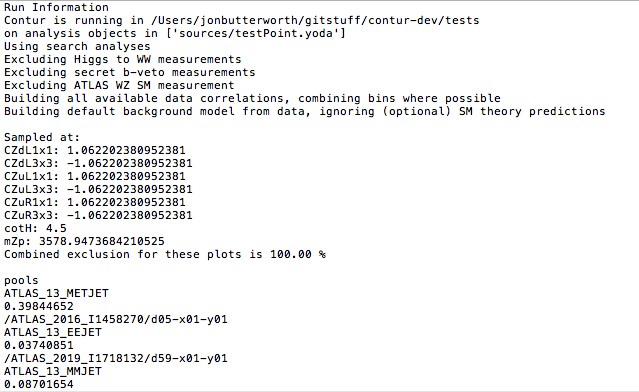
\includegraphics[scale=0.6]{plots/single_yoda_run.png}
\caption{Example output from single yoda file contur run - txt file}
\label{fig:contur_txt_output}
\end{figure}

The grid run returns a .map file which contains a pickled  .....




\subsection{Implementing Regression Tests}


\subsection{Including Theory Runs}

\section{Unit Testing}
\subsection{Likelihood Class}
\subsection{YodaFactories Class}
\subsection{Functions}


